\chapter{Method}
% This section provides a broad overview of foundational ideas
% and background material relevant to this thesis.
% In most chapters of this thesis, we include a deeper
% discussion of the related literature relevant to
% that material.




\section{Internet Explorer: An Online Agent}
% Ultimately, the goal of self-supervised learning is to learn a representation that is useful for a specific target dataset. 
% The most widely used application of machine learning is supervised learning with a known task and training dataset. 
% Practitioners typically try to improve model performance on a known target dataset by collecting additional labeled data or by fine-tuning a general-purpose pre-trained model. However, collecting data can be cumbersome and expensive, and general-purpose models may not be relevant enough to the task at hand. 
% We aim to improve performance for a known task by autonomously collecting more useful unlabeled data from the Internet. 
% With a known dataset,

We focus on the problem of efficiently improving representations for some target dataset by acquiring Internet data.
% improving performance on some prespecified task with a corresponding image dataset.
We make as few assumptions as possible and assume that we have only unlabeled training data from the target dataset. 
Successful representation learning in this setting would lead to better performance on the target dataset distribution for standard tasks like classification and detection, as well as others where the labels are not semantic (e.g., depth prediction or robotics).
% We can apply self-supervised methods directly to the target dataset, but performance quickly saturates, especially if the target dataset is small.
% We thus prioritize selectively collecting the data that is expected to improve the current model's performance on the target task. 
% Since we have a known target dataset, we can prioritize collecting data that is expected to be helpful for this task. We make as few assumptions as possible and assume that we have only unlabeled training data from the target domain, without any labels or information about what the dataset is about.
An overview of the Internet Explorer method is depicted in Figure~\ref{fig:method} and described in Algorithm~\ref{alg:internet_explorer}.
% }

\begin{figure}[t]
    \centering
    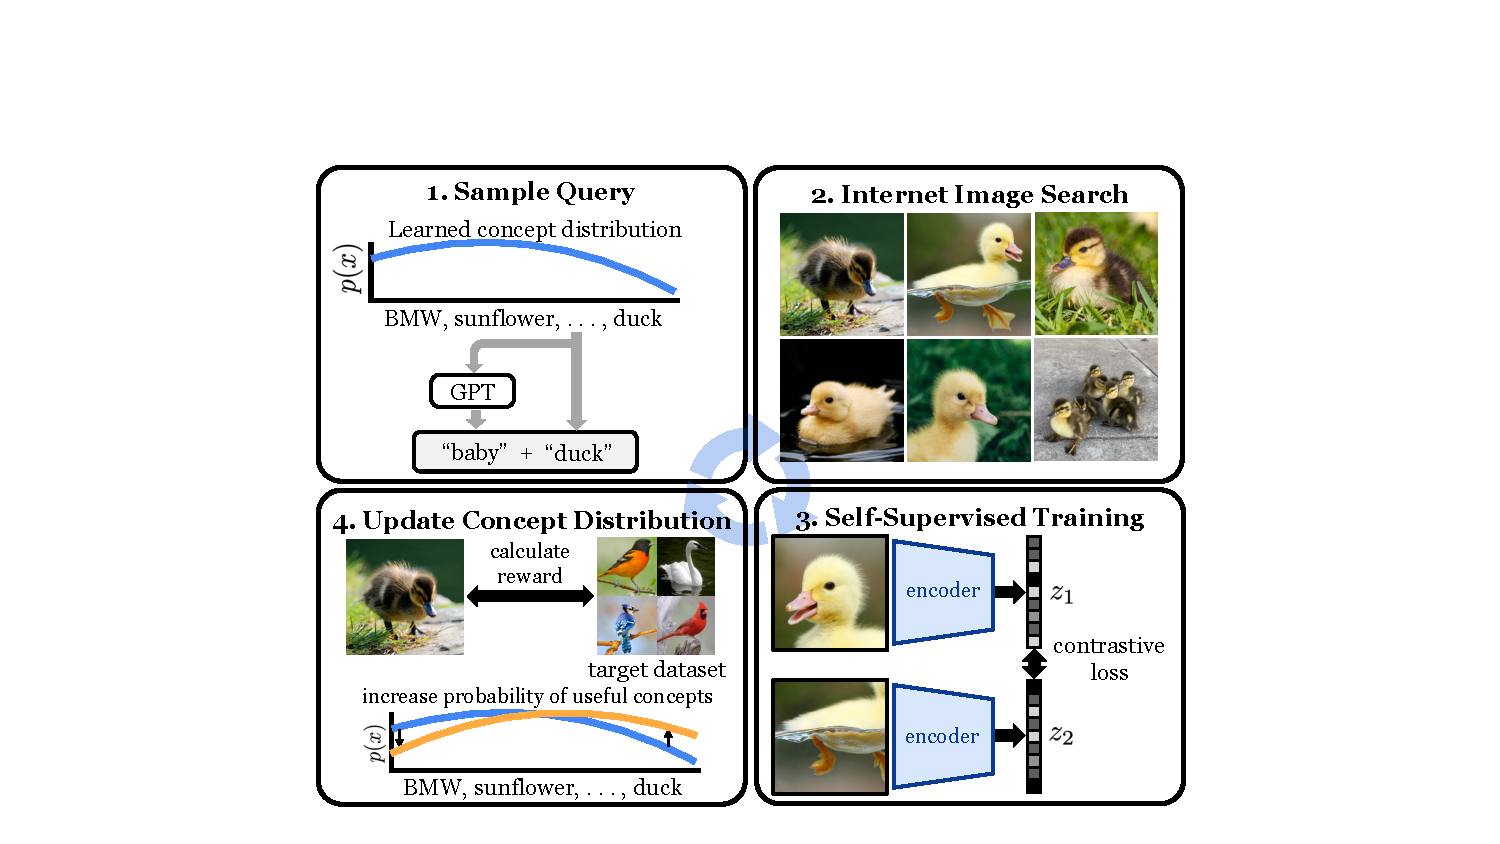
\includegraphics[width=0.8\linewidth]{figures/method_fig2.pdf}
    \caption{\textbf{Overview of Internet Explorer.} Our goal is to efficiently search the Internet for images that improve our performance on a target dataset.
        In each iteration, we first generate text queries by combining a concept sampled from a learned distribution with a GPT-generated descriptor (\S\ref{subsec:text_query_generation},~\ref{subsec:tiering}). Next, we query search engines with the resulting phrase and download the top 100 image results (\S\ref{subsec:text_to_image_search},~\ref{subsec:search_engine_main}). We add these images to the set of previously downloaded images and perform self-supervised training on the combined dataset (\S\ref{subsec:ssl}). Finally, we evaluate the relevance of the new images and update our concept distribution to increase the likelihood of similar queries if their images were similar to the target dataset (\S\ref{subsec:image_rel_reward},~\ref{subsec:unseen_reward}).
    }
    \label{fig:method}
\end{figure}

\begin{algorithm}[t]
    \caption{$\texttt{Internet Explorer}$}
    \label{alg:internet_explorer}
\begin{algorithmic}[1]
    % \State {\bfseries Input:} target dataset $\mathcal D$, SSL algorithm $\mathbb{A}$, search engine $\texttt{SE}$, encoder $f: \mathbb{R}^{H \times W \times 3} \rightarrow \mathbb{R}^d$, image reward function $r$, vocabulary $\mathcal V = \{c_i\}_{i=1}^C$, $\#$ concepts/itr $M$, $\#$ query results/search $Q$, 
    % GPT-based concept $\rightarrow$ descriptor function $\texttt{GPTDesc}$, 
    % concept distribution function $\texttt{CalcProb}$
    \State {\bfseries Input:}
    \Statex \quad target dataset $\mathcal D$
    \Statex \quad SSL algorithm $\mathbb{A}$
    \Statex \quad search engine $\texttt{SE}$
    \Statex \quad encoder $f: \mathbb{R}^{H \times W \times 3} \rightarrow \mathbb{R}^d$
    \Statex \quad image reward function $r$
    \Statex \quad vocabulary $\mathcal V = \{c_i\}_{i=1}^C$, where $C$ is $\#$ concepts
    \Statex \quad $\#$ concepts/itr $M$
    \Statex \quad $\#$ query results/search $Q$
    \Statex \quad GPT-based concept $\rightarrow$ descriptor function $\texttt{GPTDesc}$
    \Statex \quad concept distribution function $\texttt{CalcProb}$
    \State Initialize replay buffer $\mathcal{B} \leftarrow \emptyset$
    \State Initialize concept distribution $p = \text{Uniform}\{1, C\}$
    \For{iteration $=1, 2, \dots$}
        \For{$i = 1, \dots, M$}
            \State Sample concept $c_i \sim p(\mathcal{V})$ \hfill (\S\ref{subsec:text_query_generation})
            \State Sample descriptor $d_i \gets \texttt{GPTDesc}(c_i)$ \hfill (\S\ref{sec:gptj-descriptors})
            \State Image search $\{I_j^i\}_{j=1}^Q  \leftarrow \texttt{SE}(d_i + c_i, Q)$ \hfill (\S\ref{subsec:text_to_image_search})
            % \State Calculate image rewards $r(f, \mathcal D, I_j^i)$
            % \State Calculate concept reward from image rewards
            % \State Calc.\ image rewards $\{r_{\text{img},j}^i\}_{j=1}^Q \gets r(f, \mathcal D, I_j^i)$
            % \State Calc.\ concept reward $r^i_{\text{concept}} \gets \frac 1 Q \sum_{j=1}^Q r_{\text{img},j}^i$
            \State Calc.\ reward $r_{c_i} \gets \frac 1 Q \sum_{j=1}^Q r(f, \mathcal D, I_j^i)$ \hfill (\S\ref{subsec:image_rel_reward})
        \EndFor
        \State $\mathcal B_{\text{new}} = \{I_j^1\}_{j=1}^Q \cup \dots \cup \{I_j^M\}_{j=1}^Q$
        \State SSL training: $\mathbb{A}(f, \mathcal D \cup \mathcal B \cup \mathcal B_{\text{new}})$ \hfill (\S\ref{subsec:ssl})
        \State Add to buffer: $\mathcal{B} \leftarrow \mathcal{B} \cup \texttt{Top50\%}(\mathcal B_{\text{new}}, r)$  % need to align r / r_concept to r_{c_i} above
        \State Predict all concept rewards $\mathbf{r}_{\text{concept}}$ from $\{r_{c_i}\}$ \hfill (\S\ref{subsec:unseen_reward})
        \State Update concept dist $p \leftarrow \texttt{CalcProb}(\mathbf{r}_{\text{concept}})$ \hfill (\S\ref{subsec:tiering})
    \EndFor
\end{algorithmic}
\end{algorithm}

\subsection{Text-to-image Search}
\label{subsec:text_to_image_search}
% We would like a straightforward way to discover and download images from the full breadth of the Internet. 
% One directed approach to finding images online could be to progressively crawl the Web and prioritize which hyperlinks to expand based on some notion of ``usefulness''~\cite{kontogiannis2021tree}.
% However, this method has several major drawbacks. Ranking low-level hyperlinks (which of these web pages should I visit next) based on high-level semantic commands (I'd like to see pictures of Chihuahuas) is difficult to learn efficiently. Furthermore, each hyperlink expansion likely only yields a few new images, which almost certainly are not relevant to the concepts we care about. 
We discover and download images from the full breadth of the Internet by querying text-to-image search engines, which return images based on their captions and surrounding text. Text-to-image search is fast, returns diverse images from across the Internet, and enables searches for vastly different queries simultaneously. Note that text-to-image search is noisy and makes use of weak supervision (the image-text pairing on webpages). Thus, we only perform self-supervised training on the downloaded images. We use a public codebase to query Google Images, which can download the top 100 images for each query~\cite{hardikvasa, Joeclinton1}. We also try other search engines in \cref{subsec:search_engine_main}.
% We turn on SafeSearch, mark preference for photographs, and set the minimum image size to 350, the smallest setting available. 
% should we show an example of noisy results?

\subsection{Text Query Generation}
\label{subsec:text_query_generation}
% TODO: explain why a lot of thought goes into the query model. 
As text queries are our only input interface with the Internet, it is crucial that we can generate diverse queries that correspond to a variety of visual categories. Specificity is also important. Once a useful visual category is identified, generating fine-grained variants of the query is necessary to obtain data for all visual variations in the category.
% Language models could potentially be used to produce text queries, and reinforcement learning could be used to adjust their behavior based on the curiosity reward. Previous work found that RL worked well for preference-based training from human feedback~\cite{ziegler2019fine,stiennon2020learning,nakano2021webgpt}. However, we found that models such as BERT~\cite{devlin2018bert} or GPT-2~\cite{radford2019language} preferred generating human-centric phrases and did not generate sufficiently visually diverse queries, even with extensive prompt tuning. Thus, we avoid language models and 
We construct queries by combining two components: 
\begin{enumerate}[noitemsep,topsep=0pt]
    \item \textit{Concepts} specify semantic categories such as people, places, or objects. % Examples: golden retriever, daisy, BMW. 
    \item \textit{Descriptors} are modifiers that generate variations in appearance. % Examples: big, narrow, red. 
\end{enumerate}

We draw our concepts from the WordNet hierarchy~\cite{miller1995wordnet}, which consists of $146{,}347$ noun lemmas. Not all of these lemmas are visual, but the vocabulary still covers an incredible range of topics (see examples in \cref{sec:wordnet_lemmas}).
To generate a text query, we first sample a concept from a learned distribution over our vocabulary. This discrete distribution is defined by our estimates of how relevant each concept in the vocabulary is at the current time (see \cref{subsec:image_rel_reward} for details on estimating rewards and \cref{subsec:tiering} for the distribution).
Given a sampled concept, we can generate a descriptor by prompting a GPT-J language model~\cite{gpt-j} with examples of descriptor-concept pairs (details and examples in \cref{sec:gptj-descriptors}).
Finally, as shown in Step 1 of \cref{fig:method}, we simply concatenate the concept and descriptor. If our concept is ``duck'' and the GPT-generated descriptor is ``baby,'' our search engine query will be ``baby duck''.


\subsection{Self-supervised Training}
\label{subsec:ssl}
% EB NOTE:
% this section currently reads as: we use SSL, simsiam didnt work, but we use moco. moco details. we can also use other methods too
% IMO a potentially stronger stance: SSL is the core of our method, and it is compatible with any SSL algo and across many modalities. we choose images for X reason and moco for Y reason. then moco details

We use self-supervised learning (SSL) to learn useful representations from the unlabeled images that we download from the Internet. 
% We experimented with using SimSiam~\cite{chen2020exploring} as our base SSL algorithm due to its simplicity (no temperature, EMA rate, or loss weighting terms to tune), but found that it was unstable to train~\cite{li2022understanding}. 
Internet Explorer is compatible with any SSL algorithm that uses images or image-text pairs, including contrastive~\cite{he2020momentum,chen2020simple}, non-contrastive~\cite{grill2020bootstrap,zbontar2021barlow,bardes2021vicreg,caron2021emerging}, masking-based~\cite{bao2021beit,he2022masked}, or multimodal~\cite{radford2021learning} approaches. 
For speed and stability reasons, we use the MoCo-v3 algorithm~\cite{chen2021empirical}, which trains encoders $f_q$ and $f_k$ on augmentations $(x_1, x_2)$ of the same image to output vectors $q = f_q(x_1)$ and $k = f_k(x_2)$. $f_q$ is trained to minimize the InfoNCE loss~\cite{oord2018representation}:
\begin{align}
    \mathcal L_q = -\log \frac{\exp(q \cdot k^+ / \tau)}{\exp (q \cdot k^+ / \tau) + \sum_{k^-} \exp (q \cdot k^- / \tau) }
    \label{eq:moco_loss}
\end{align}
where $k^+$ corresponds to $f_k$'s output on the other augmentation of the image used to compute $q$, and the set of negative examples $\{k^-\}$ corresponds to $f_k$'s output on other images in the batch. The temperature $\tau$ is set to $1$ by default. $f_k$ consists of a base encoder, a projection MLP, and a prediction head, whereas $f_q$ is the exponential moving average of the base encoder and projection MLP from $f_k$. By training $q$ and $k^+$ to be similar across image augmentations, MoCo-v3 encourages the network to learn high-level semantic features. 

% In each iteration of our method, we use MoCo-v3 to fine-tune a ResNet-50 model~\cite{he2016deep} on a mixture of newly downloaded, previously downloaded, and target dataset images.
% Before turning to the Internet, we initialize our model using a MoCo-v3 checkpoint trained offline for 100 epochs on ImageNet and then
% another X steps on a mixture of ImageNet and the target dataset images. 
% fine-tuned with MoCo-v3 on the target dataset. Without using labels, we select the starting checkpoint for Internet Explorer by early-stopping on the SSL loss, which highly correlates with target accuracy~\cite{li2022understanding}.

Before turning to the Internet, we initialize a ResNet-50 model~\cite{he2016deep} using a MoCo-v3 checkpoint trained offline for 100 epochs on ImageNet and then fine-tuned on the target dataset. Without using labels, we select the best starting checkpoint by early stopping on the SSL loss, which highly correlates with target accuracy~\cite{li2022understanding}.
In each iteration of our method, we use MoCo-v3 to fine-tune on a mixture of newly downloaded, previously downloaded, and target dataset images.
% another X steps on a mixture of ImageNet and the target dataset images. 


% Even though we focus on using MoCo-v3, note that Internet Explorer is compatible with any SSL algorithm that uses images or image-text pairs, including contrastive~\cite{he2020momentum,chen2020simple}, non-contrastive~\cite{grill2020bootstrap,zbontar2021barlow,bardes2021vicreg,caron2021emerging}, masking-based~\cite{bao2021beit,he2022masked}, or multimodal~\cite{radford2021learning} approaches. 

\subsection{Image Relevance Reward}
\label{subsec:image_rel_reward}
We want to rank newly downloaded images by how much they improve our features for the target dataset. This allows us to (a) prioritize taking gradient steps on useful images, and (b) understand what to search for in subsequent iterations. Unfortunately, it is challenging to directly measure the effect of an individual training example on performance. Numerous techniques have been proposed~\cite{koh2017understanding,feldman2020neural,paul2021deep,ilyas2022datamodels}, but they all require extensive and repeated training on new images to estimate their impact. 

% Instead of trying to precisely measure what is learned from each image, we rank the images by their distance in representation space to the target dataset images. The images most similar to the target dataset induce larger contrastive loss, since each $\exp(q \cdot k^-)$ term in the denominator of Eq.~\ref{eq:moco_loss} is larger when the negative examples $\{k^-\}$ are closer to $q$.
Instead of trying to precisely measure what is learned from each image, we use its similarity to the target dataset as a proxy for being relevant to training.
We rank the downloaded images by their similarity in representation space to the target dataset images; those most similar to the target dataset induce larger contrastive loss since each $\exp(q \cdot k^-)$ term in the denominator of Eq.~\ref{eq:moco_loss} is larger when the negative examples $\{k^-\}$ are closer to $q$.
These ``hard negatives''~\cite{robinson2020contrastive,schroff2015facenet,oh2016deep,harwood2017smart,wu2017sampling,ge2018deep} yield larger and more informative gradients and should result in the biggest improvement in representation quality.
% The best way to improve performance on the target dataset is by finding data that \textit{looks like the target dataset.} Figure~\ref{fig:in_vs_flowers} shows that self-supervised learning on just 2040 Flowers102 images outperforms self-supervised pre-training on ImageNet, which contains 1.2 million images ($628\times$ as much data). Pre-training on only flower images only requires about 2\% the training time as ImageNet pre-training.
% Motivated by this, 
% We heuristically want to find Internet images similar to the ones in the target dataset, in hopes that they most efficiently improve self-supervised training. Thus, we formulate a curiosity reward (higher is better) to prefer images that are most similar in representation space to the target dataset images.
% We want to find the best Internet images for future self-supervised training. 
% As shown in Figure~\ref{fig:curiosity_reward}, the curiosity reward for a particular image is its representation's negative distance to its closest neighbor in the target dataset.
Thus, overloading notation for $k$, we compute the reward for a particular image as its representation's average cosine similarity to its $k$ closest neighbors in the target dataset. Given an image encoder $f_k: \mathbb{R}^{H\times W\times 3} \rightarrow \mathbb{R}^d$, an unlabeled target dataset $\mathcal D = \{ x_i \}_{i=1}^N$, and a new image $y$ to evaluate, the reward is calculated:
\begin{align}
    r(f_k, \mathcal D, y) =
        \max_{\substack{I \subset \{1, \ldots, N\}; \\ |I| = k}}
        \frac{1}{k} \sum_{i \in I} S_{\cos}\left(f_k(x_i), f_k(y)\right)
\end{align}
where $S_{\cos}$ is the cosine similarity. A previous metric for identifying relevant data~\cite{jiang2021improving} used $k=1$ nearest neighbors, 
% but we found that this was too noisy and enabled high rewards for images unrelated to almost all of the target dataset. 
but we found that this was too noisy and allowed high rewards for outlier target images to distract our search.
We instead use $k=15$ to improve the accuracy of our relevance estimation.
In \cref{subsec:reward_analysis}, we compare our reward to alternatives and explore their failure modes. This reward is used for two purposes: determining which of the downloaded images to train on and, subsequently, which concepts would be useful to search for next.

\vspace{-0.06in}
\paragraph{Which images to train on.}
Many newly downloaded images are not worth training on, since they come from unrelated queries or are noisy results from the search engine.
Thus, at the end of each iteration, we rank the newly downloaded images by their reward and save the top $50\%$ to a replay buffer that we maintain across iterations. In subsequent iterations, we continue training on this filtered data.

\vspace{-0.06in}
\paragraph{Determining which concepts are useful.}
When we search for a concept and get back $Q$ image results $\{ I_i \}_{i=1}^Q$, we take the average of the top 10 image-level rewards $r_i = r(f_k, \mathcal D, I_i)$ and use that as a \textit{concept-level score}. This gives us an accurate measure of the relevance of a particular query and reduces the impact of noisy search results. 



\subsection{Estimating Reward for Unseen Concepts}
\label{subsec:unseen_reward}

\subsubsection{Concept Embeddings}
Since our vocabulary contains hundreds of thousands of concepts, it would be inefficient to test whether \emph{each} possible query yields relevant images. Luckily, we can estimate the quality of queries by using the observed rewards of the queries searched so far. Humans can do this effortlessly due to our understanding of what each concept means. To us, it is obvious that if querying ``duck'' yielded useful images for this dataset and ``BMW'' did not, then we should search for more images of animals and not cars. We want to give our method the same understanding of concept meaning, so we embed our $146{,}347$ WordNet concepts into a 384-dimensional space using a pre-trained sentence similarity model~\cite{reimers2019sentence}. We provide relevant context about each concept to the text embedding model by using additional information from WordNet in the following template:

\begin{quote}
    {\tt {\small \{lemma\} (\{hypernym\}): \{definition\}}}
\end{quote}
For example, the text that is embedded for the concept ``Chihuahua'' is:

\begin{quote}
    {\tt {\small Chihuahua (toy dog): an old breed of tiny short-haired dog with protruding eyes from Mexico held to antedate Aztec civilization.}}
\end{quote}


\subsubsection{Predicting Rewards}
Now that we have a representation of each concept, we can estimate the reward for untried concepts by using the rewards of concepts that we have already searched for.
We use Gaussian process regression (GPR)~\cite{williams1995gaussian} over the text embeddings $\{\mathbf{e}_i\}$ to predict the concept-level reward $r(\mathbf{e}_i)$ for untried concepts. 
GPR models the function outputs for any set of inputs $\{r(\mathbf{e}_i)\}$ as jointly Gaussian random variables. 
The covariance of any two variables $r(\mathbf{e}_i)$ and $r(\mathbf{e}_j)$ is determined by the kernel $k(\mathbf{e}_i, \mathbf{e}_j)$, which we set as the default RBF kernel $k(\mathbf{e}_i, \mathbf{e}_j) = \exp(\frac{-\|\mathbf{e}_i - \mathbf{e}_j\|_2}{2})$. 
Given the observed rewards for concepts $R_{obs} = \{r(\mathbf e_i)\}$, GPR calculates the posterior distribution over the rewards for an unobserved concept $\mathbf e'$, $P(r(\mathbf e') \mid \{r(\mathbf{e}_i)\} = R_{obs})$. Given that the joint distribution  $P(\{r(\mathbf{e}_i)\}, r(\mathbf{e}'))$ is Gaussian, the posterior is also Gaussian with mean $\mu(\mathbf e')$ and variance $\sigma{(\mathbf e')}^2$. The locality provided by the RBF kernel enables reasonable reward predictions, and having a distribution over rewards instead of a point estimate allows us to explore potentially good concepts. We encourage exploration by setting the score of unobserved concepts to $\mu(\mathbf{e}_i) + \sigma(\mathbf{e}_i)$.

% a practical issue: GPR slows down a ton as the number of points increases. for this reason, after 10 iterations (256 queries * 100 images * 10 iters = 256k points), we switch to a simple ridge regression model. this is a good tradeoff because we have a lot of data by this point, and we don't need to explore as much anymore.

A practical issue is that GPR does not scale well to large numbers of points, and fitting the model after each iteration becomes prohibitively slow. To address this, we use GPR for the first 10 iterations ($256$ queries $\times$ $100$ images $\times$ $10$ iterations $\approx 256{,}000$ points), and then switch to a simple ridge regression model that predicts solely the mean rewards $\mu(\mathbf{e}_i)$---and thus we eliminate the exploration term $\sigma(\mathbf{e}_i)$ from the reward prediction. This is a good tradeoff because we have a lot of data by this point, and we don't need to explore as much anymore.
The number of iterations at which we switch to ridge regression is a hyperparameter that can be tuned to balance exploration and exploitation + speed. We found that 10 iterations to work well in practice.


\subsection{Query sampling distribution}
\label{subsec:tiering}

\begin{figure}[t]
    \centering
    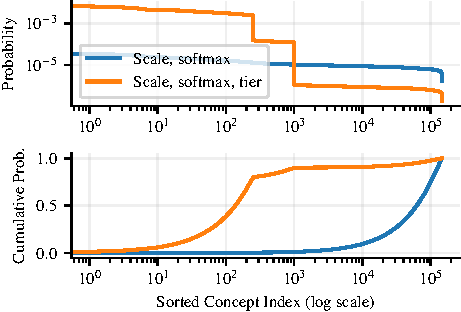
\includegraphics[width=0.7\linewidth]{figures/sampling_dist_shorter.pdf}
    \caption{\textbf{Learned concept sampling distribution.} Given estimated scores for each of the $146{,}347$ concepts, we need to choose how often to sample each one in order to balance exploration and exploitation.
    \textbf{Top:} we scale our scores to a desired temperature, then take the softmax to obtain a distribution over concepts. Finally, we create tiers so that the top 250 concepts have $80\%$ of the probability mass, and the next 750 have $10\%$. This ensures that we sample enough from the top $1{,}000$ concepts while still exploring other concepts with lower scores.
    \textbf{Bottom:} the top 1000 concepts are only sampled a tiny fraction of the time without tiering.}
    \label{fig:sampling_dist}
    \vspace{-0.12in}
\end{figure}

Once we have estimates for the quality of each concept, how do we determine what to search for next?
% We have two desiderata: 
    % \begin{enumerate}
%     \item Sufficient exploration of potentially good queries. 
%     % \item Sample the top concepts frequently enough, so that we get enough relevant training data for SSL. 
%     \item Frequent enough sampling of the top concepts, so that we get good relevant training data for SSL. 
% \end{enumerate}
We face the age-old dilemma of exploration versus exploitation:
% \begin{enumerate}[noitemsep,topsep=0pt]
%     \item We need to sample the top concepts frequently enough to get relevant training data for SSL.
%     \item At the same time, we need sufficient exploration of promising untried concepts.
% \end{enumerate}
we need to sample the top concepts frequently enough to get relevant training data for SSL, while at the same time, we need sufficient exploration of promising untried concepts.
% A greedy approach, like only searching for the top $C$ concepts with the highest estimated reward, results in poor exploration of untried concepts. Instead, w

We use a sampling-based approach based on Boltzmann exploration~\cite{sutton1991dyna}. Boltzmann exploration samples based on a scaled softmax distribution $ p(c_i) \propto \exp(r(c_i)/\tau)$, where  
% maybe make reference to bandits, ucb, bayesian optimization, soft q learning 
% \begin{align}
%     p(c_i)  = \frac{\exp(r(c_i)/\tau)}{\sum_j \exp(r(c_j)/\tau)}
% \end{align}
$\tau$ is the temperature scaling.
However, with a large vocabulary (action space) of $146{,}347$ concepts, it becomes difficult to tune $\tau$ so that we sample the top concepts frequently enough without being too skewed. 
Thus, we define a ``tiering function'' to adjust the probability mass in specified intervals of our distribution. Given a sorted discrete probability distribution $p$, interval boundaries $T_0 =0 < T_1 < \dots < T_n$, and interval masses $\Delta_0, \dots, \Delta_{n-1}$ such that $\sum_i \Delta_i = 1$,  tiering computes a new distribution: 
\begin{align}
    p_i^{\text{tier}} = \Delta_j \frac{p_i}{\sum_{k=T_j}^{T_{j+1}} p_k} \;\;\; \text{for } j \text{  s.t.  }T_j \leq i < T_{j+1} 
\end{align}
$p^{\text{tier}}$ is a new distribution such that $\sum_{k=T_j}^{T_{j+1}} p^{\text{tier}} = \Delta_j$. We use $T_0=0$, $T_1=250$, $T_2=1{,}000$, $T_3=146{,}347$, $\Delta_0=0.8$, $\Delta_1 = 0.1$, and $\Delta_2=0.1$.
Simply put: we give the highest-ranked $250$ concepts $80\%$ of the probability mass, the next $750$ concepts $10\%$, and all remaining concepts $10\%$.
Figure~\ref{fig:sampling_dist} shows that tiering the scaled softmax distribution samples frequently enough from the top concepts while a vanilla scaled softmax distribution does not.
Note that the untiered distribution would sample the top $1000$ concepts only $\approx 0.1\%$ of the time, while the tiered distribution samples them $90\%$ of the time.

% Things to mention 
% \begin{itemize}
%     \item comparison of different ways of computing the text embeddings. describe just embedding the concepts, vs embedding the concept and the wikipedia summary
%     \item histograms of the text embedding similarity
%     \item ways of purifying the similarity matrix
%     \item TODO: think about rewarding quality over quantity
% \end{itemize}

\subsection{Provable speedup in relevant query identification}
\label{subsec:provable_speedup}
We now show that our method can provably speed up the time to identify all relevant concepts in a dataset.
Assume that our vocabulary of $n$ concepts contains $c \cdot s \ll n $ relevant concepts, which are partitioned into $c$ disjoint clusters of size $s$. We want to discover every relevant concept by sampling concepts uniformly at random (with replacement) to test. Assume that sampling a concept conclusively tells us whether it is relevant. Furthermore, assume that we could optionally use a Gaussian process regression model which, if we've sampled a relevant concept, tells us that all the concepts in its cluster are also relevant.\\

\begin{restatable}{lemma}{lemmaspeedup}
    \label{lemma:speedup}
    Let $T_{base}$ be the expected time to identify every relevant concept without the GPR, and $T_{GPR}$ be the expected time when exploiting the additional knowledge from the GPR. Then, $T_{base} = n H_{c \cdot s}$, $T_{GPR} = \frac{nH_{c}}{s}$, and the speedup from GPR is $\frac{T_{base}}{T_{GPR}} \approx s \log s$.
\end{restatable}

\begin{proof}
    This problem is a variant of the coupon collector problem. Let's first compute $T_{base}$ as the sum of expected times $t_i$ to identify the next relevant concept. 
    \begin{align}
        T_{base} &= \sum_{i=1}^{cs} t_i \\
                 &= \sum_{i=1}^{cs} \frac{1}{p_i} \\
                 &= \sum_{i=1}^{cs} \frac{n}{cs + 1 - i} \\
                 &= n \sum_{i=1}^{cs} \frac{1}{cs + 1 - i} \\
                 &= n H_{cs}
    \end{align}
    where $H_{cs}$ is the $cs$th harmonic number. Similarly, we can compute $T_{GPR}$ as the sum of expected times $t_i$ to identify the next relevant cluster.  
    \begin{align}
        T_{GPR} &= \sum_{i=1}^{c} t_i \\
                 &= \sum_{i=1}^{c} \frac{1}{p_i} \\
                 &= \sum_{i=1}^{c} \frac{n}{s (c + 1 - i)} \\
                 &= \frac{n}{s} \sum_{i=1}^{c} \frac{1}{c + 1 - i} \\
                 &= \frac{nH_{c}}{s}
    \end{align}
    The speedup is then $\displaystyle \frac{T_{base}}{T_{GPR}} = s \frac{H_{cs}}{H_c} \approx s \log s$.
\end{proof}

We find that in practical settings (e.g., the Pets example analyzed in Fig.~\ref{fig:reward_over_training}), we can accurately predict how many samples are required to discover all useful concepts. If the vocabulary size is $n \approx 150{,}000$, the number of clusters is about $c = 2$ (one for cats and one for dogs), and the size of each cluster is about $150$, then $T_{GPR} = 1500$, which roughly matches the $9 \times 256 = 1792$ queries it took to discover both cats and dogs in the Pets dataset.


\section{Method Details}

% We draw our concepts from the WordNet hierarchy~\cite{miller1995wordnet}, which consists of $146{,}347$ noun lemmas. Not all of these lemmas are visual, but the vocabulary still covers an incredible range of topics.
% % For reference, here are 6 randomly sampled concepts:  {\tt {\small `sleep talking', 
% % `beach wagon', `Balearic Islands', `borosilicate', `genus Loranthus', `humpback whale'}}.
% We can generate descriptors for each concept by prompting a GPT-J language model~\cite{gpt-j} with examples of descriptor-concept pairs (details in the supplementary).
% % For reference, here are 7 randomly sampled descriptors for ``labrador retriever'': {\tt {\small `friendly', `short', `long-legged', `big', `fast', `blue-eyed', `handsome'}}.

\subsection{WordNet Lemmas}
\label{sec:wordnet_lemmas}
We draw our concepts from the WordNet hierarchy~\cite{miller1995wordnet}, which consists of $146{,}347$ noun lemmas. For reference, here are 32 randomly sampled concepts:
\begin{quote}
{\tt { 
% `sleep talking', `beach wagon', `Balearic Islands', `borosilicate', `genus Loranthus', `humpback whale'
"resolution",
"lodgment",
"phycobilin",
"acidosis",
"widening",
"human face",
"family Crassulaceae",
"sail",
"Ipomoea imperialis",
"Davis",
"prothrombin",
"cease",
"marsh clematis",
"major power",
"chump change",
"madcap",
"junky",
"pere david's deer",
"make-up",
"genus Rumex",
"gape",
"Brachychiton populneus",
"bell morel",
"wain",
"friendly",
"Principe",
"bottle green",
"glycerol trimargarate",
"water-shield",
"San Joaquin River",
"woodsman",
"pin".
}}
\end{quote}

\subsection{GPT-J Descriptor Prompting}
\label{sec:gptj-descriptors}
We use GPT-J-6B~\cite{gpt-j}, a free, open-source autoregressive language model, to generate useful descriptors for a given concept. We use the following prompt template: 
\begin{itemize}
    \item[] \texttt{"What are some words that describe the quality of `\{concept\}'?} 
    \item[] \texttt{The \{concept\} is frail.}
    \item[] \texttt{The \{concept\} is red.}
    \item[] \texttt{The \{concept\} is humongous.}
    \item[] \texttt{The \{concept\} is tall.}
    \item[] \texttt{The \{concept\} is"}
\end{itemize}

We sample completions with a temperature of 0.9 and a max length of 100 tokens. We truncate the completion after the first comma, period, underscore, or newline character (including the special character). If the truncated completion is degenerate and contains a duplicate of the concept, we resample another completion. After successfully sampling a descriptor, we prepend it to the concept and use the resulting phrase as our search query. 

% - TODO: put in a page of examples.   
% - Pencil: 'fragile', 'huge!', 'too big', 'colorful', 'dark', 'too soft', 'blunt', 'narrow', 'round', 
% 'blue', 'black', 'a soft piece of wood', 'thick', 'heavy', 'light', 'short'
% - TODO: These descriptors generally 
% - Our prompt can be easily 

For reference, here are 32 randomly sampled descriptors for ``labrador retriever'':
% {\tt {\small `friendly', `short', `long-legged', `big', `fast', `blue-eyed', `handsome'}}.
\begin{quote}
{\tt { 
% `sleep talking', `beach wagon', `Balearic Islands', `borosilicate', `genus Loranthus', `humpback whale'
"a good-looking dog",
"very gentle",
"a",
"brown",
"lovable",
"a strong runner",
"a male or a female",
"sturdy",
"agile",
"a strong",
"beautiful",
"a male",
"kind",
"long-haired",
"a male or a female",
"a good-looking dog",
"gentle",
"medium",
"loyal",
"very gentle",
"blue-eyed",
"sturdy",
"blue-eyed",
"a retriever",
"kind",
"loyal",
"large",
"brown",
"good-natured",
"gentle",
"large",
"small".
}}
\end{quote}



\subsection{Concept Vocabulary Size}
\label{sec:concept_vocab_size}
As stated in \cref{subsec:text_query_generation}, our vocabulary comprises the $146{,}347$ noun lemmas in the WordNet hierarchy. Thus, in all our experiments, Internet Explorer only searches for WordNet terms (plus the class names, if we have knowledge of the label set). We found that this worked quite well for these standard benchmarks. Note that expanding the vocabulary (e.g., adding technical terms relevant to a specific topic) can easily be done by adding those terms to the list of possible concepts. One easy extension would be to add page titles and frequent unigrams and bigrams from Wikipedia, as was done to generate the CLIP training set~\cite{radford2021learning}. Doing so would expand our vocabulary to roughly $500{,}000$ total concepts. 

\subsection{Query Model Details}
\label{sec:query_model_details}
\paragraph{Temperature for concept distribution}
After estimating scores $r(c_i)$ for each concept $c_i$, we do a temperature-scaled softmax, followed by the tiering operation described in \cref{subsec:tiering}. We compute the temperature $\tau$ such that 
\begin{align}
     \text{SMR} = \frac{\max_i r(c_i) - \min_i r(c_i)}{\tau}
\end{align}
where the ``softmax range'' $\text{SMR} \in \mathbb R$ is the desired gap between the largest and smallest scores after temperature scaling. After the softmax $p(c_i) \propto \exp(r(c_i) / \tau)$, the softmax range determines the likelihood ratio of most likely concept to least likely concept: 
\begin{align}
    \frac{\max_i p(c_i)}{\min_i p(c_i)} &= \frac{\max_i \exp(r(c_i) / \tau)}{\min_i \exp(r(c_i) / \tau)} \\
      &= \exp \left(\frac{\max_i r(c_i) - \min_i r(c_i)}{\tau}\right) \\
    &= \exp(\text{SMR})
\end{align}
Thus, SMR is an easy way to specify the relative likelihood of the highest and lowest scoring concepts and achieve a desired exploration-exploitation balance. 


\paragraph{Label set-guided vocabulary}
To reduce our search space in the label set-guided setting, in which we know the English names of the classes a priori, we generate a subset of the WordNet vocabulary that contains only the top-$10\%$ most semantically-relevant concepts to each target dataset.
We use a pre-trained text embedding model~\cite{reimers2019sentence} to generate $384$-dimensional embeddings for each concept in WordNet, using the same template described in \cref{subsec:unseen_reward}

\begin{quote}
{\tt {\small \{lemma\} (\{hypernym\}): \{definition\}}}.
\end{quote}

To generate a similar embedding for concepts in target datasets, we use the summary from Wikipedia in place of the definition and the ``category'' of the target dataset (shown in \cref{tab:dataset_categories}) in place of the hypernym:

\begin{quote}
{\tt {\small \{label\} (\{category\}): \{summary\}}}.
\end{quote}


\begin{table}
    \centering
    \begin{tabular}{ll}
    \toprule
        Dataset & Category \\
    \midrule
        Oxford Flowers102 & Flower \\
        Oxford IIIT Pets & Pet \\
        Food101 & Food \\
        Birdsnap & Bird \\
        VOC2007 & Object \\
    \bottomrule
    \end{tabular}
    \caption{\textbf{Target Dataset ``Category''}.
    }
    \label{tab:dataset_categories}
\end{table}

After generating the embeddings for each concept in the target dataset, we find the $k$-NN distance for each WordNet concept to the target dataset embeddings, where $k$ is chosen to be $1/3$ the size of the class label set.
We then rank the concepts in WordNet by the distance and take the closest $10\%$ of terms as our subset. This subset is used for all methods in the label set-guided setting, including the random exploration methods. 






\subsection{Training Details}
In each iteration, we download roughly 25k candidate images, since we download up to 100 images for each of the 256 queries. Given this set $\mathcal C$ of candidate images, we sample $\text{PCR} \times |\mathcal C|$ images from the union of the replay buffer $\mathcal B$ and the target dataset training images $\mathcal D$. PCR (past data to candidate data ratio) is a scalar value that determines how much old data vs new data to train on at every iteration. We set $\text{PCR}=2$ for all experiments. We perform $10$ epochs of training over the union of the new candidate data and the sampled replay buffer and target dataset images. 

\subsection{Hyperparameters}
% privilege ratio, privilege gamma 
% k 
% GP 

\cref{tab:hyperparameters} shows our hyperparameter values, which are shared across datasets. We perform minimal hyperparameter tuning and copy most of the values from the MoCo-v3~\cite{chen2021empirical} ResNet-50 configuration. 
We will also release our code upon acceptance, which we hope will clarify any remaining implementation details and make it easy for the community to reproduce and build on our work. 
\begin{table}
    \centering
    % \begin{adjustbox}{width=\linewidth}
    \begin{tabular}{ll}
    \toprule
        Hyperparameter & Value \\
    \midrule
        Architecture & Resnet-50~\cite{he2016deep} \\
        Optimizer & LARS~\cite{you2017large} \\
        Batch size & $224$ \\
        Learning rate & $0.8 \times \frac{224}{256}$ \\
        Learning rate schedule & constant \\
        MoCo momentum & $0.9985$ \\
        RandomResizedCrop min crop area & $0.2$ \\
        % PCR & 2? \\
        Queries per iteration & $256$ \\
        Requested images per query & $100$ \\
        Min images per query & $10$ \\    
        Softmax range (SMR) & $3$ \\
        PCR & $2$ \\
        Epochs per iteration & $10$ \\
    \bottomrule
    \end{tabular}
    % \end{adjustbox}
    \caption{\textbf{Internet Explorer hyperparameters}.}
    \label{tab:hyperparameters}
\end{table}


\subsection{Image Licenses}
Internet Explorer uses images that were indexed by a web crawler (Google Images and LAION) or uploaded to Flickr. The images and their rights belong to their respective owners; we use, download, and train on them under fair use guidelines for research. 

%%% Local Variables:
%%% coding: utf-8
%%% mode: latex
%%% TeX-engine: xetex
%%% TeX-master: "../thesis"
%%% End:
